\chapter{Introduction to Heavy Ion Physics}
\label{sec:concepts}
\section{The Standard Model}
\label{sec:sm}
The \gls{sm} is the current theoretical framework used to describe all microscopic processes. It contains all the known fundamental particles and describes the interactions among them via the strong, weak, and electromagnetic force. While the current formulations stems from the late 1970s, many of its concepts date back further and were developed by a joint effort of many physicists. All particles in this theory are believed to be point like, i.e.\ are fundamental. Albeit being extraordinarily successful at explaining most experimental results and predicting novel phenomena, the \gls{sm} is known to be an incomplete theory since it does neither contain a dark matter candidate nor a quantum description of gravity. An example of its success are studies of the electron magnetic moment $g/2$: The \gls{sm} prediction agree with current experimental over more than ten orders of magnitude \cite{Odom2006}. The latest and possibly most public achievement was the discovery of the Higgs boson in 2013, which was introduced to the \gls{sm} to assign masses to its particles.\\


All dynamics and kinematics of the \gls{sm} are governed by the Lagrangian $\mathcal{L}$ which may be split up into three sectors as $\mathcal{L} = \mathcal{L}_{EW} + \mathcal{L}_{QCD} + \mathcal{L}_{H}$. The following sections will explain the fields (yielding leptons, quarks and the Higgs boson) as well as the interactions (gauge bosons) between them in more detail.


\subsection{Leptons and quarks}
\label{sec:leptons-and-quarks}
\begin{figure}
  \centering
  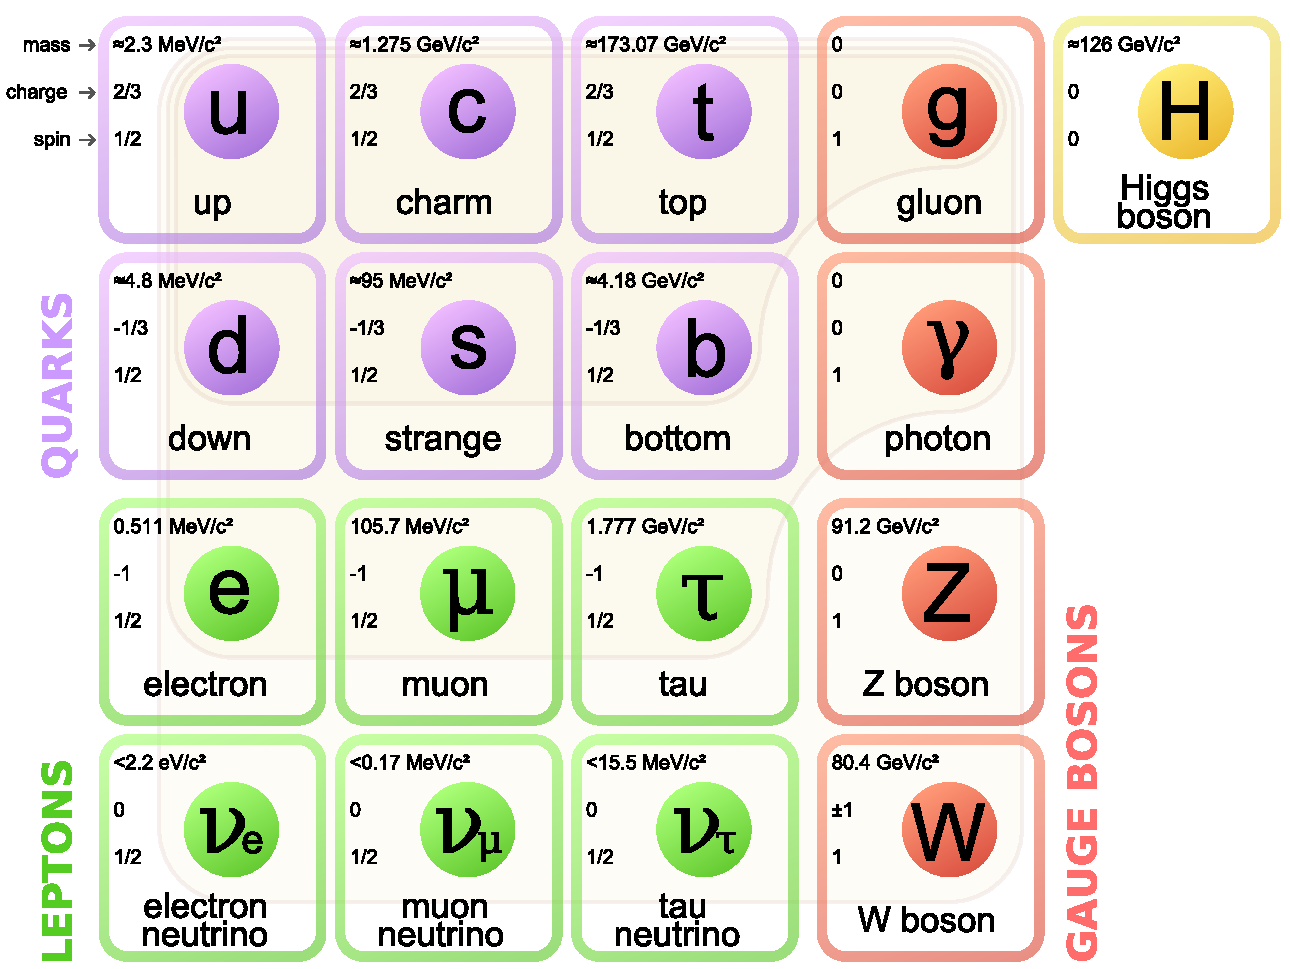
\includegraphics[width=.6\textwidth]{figures/sm-particles.pdf}
  \caption[Summary of all the fundamental particle of the Standard model.]{Summary of all the fundamental particle of the Standard model. The three families of the quarks and leptons are given by their respective column. The shaded backgrounds indicate to which fermions each gauge boson couples. From \cite{Cush2014}.}
  \label{fig:sm}
\end{figure}

All matter particles and force carriers of the standard model are depicted in fig. \ref{fig:sm}. The former are separated into leptons (green) and quarks (purple). Each is again composed of three families (often also called generations or flavors) depicted by columns in the figure. All quarks and all leptons are spin $1/2$ particles and thus fermions; however, they differ in various other properties.


Each lepton family consists of one massive particle with an electric charge $-1e$ ($e$ being the electron charge) and one neutral, very light, particle called a neutrino. The charged particles are the electron $e$, muon $\mu$ or tau $\tau$. Additionally to the electric charge, leptons carry an electron number ($L_e$), a muon number ($L_\mu$) and a tau number ($L_\tau$) which is either $1$ if the particle is a member of the respective family or $0$ otherwise.\\

The six quarks, up ($u$), down ($d$), strange ($s$), charm ($c$), bottom ($b$) and top ($t$) have masses rising in this order. $u$, $c$ and $t$ have electrical charge $2/3e$ while $d$, $s$ and $b$ are charged by $-1/3e$. A property unique to quarks is the so called color charge: each quark carries either a red, green or blue color. The implications of this quantum number is further discussed after the introduction of the force carriers in sec. \ref{sec:qcd}. 

For each lepton exists a corresponding anti-particle with the exact same mass but all the quantum numbers inverted. In case of color, the inverse is defined as ``anti-red'', ``anti-green'' and ``anti-blue''.

\subsection{The gauge bosons}
\label{sec:gauge-bosons}
From a mathematical point of view, all the particles of the \gls{sm} are described as fields and all the interaction arise from a local $SU(3)\times SU(2) \times U(1)$ symmetry of $\mathcal{L}$. In a simplified picture, this means that $\mathcal{L}$ remains unchanged if all the fields are transformed by any set of matrices from the $SU(3)\times SU(2) \times U(1)$ group. $SU(3)$ acts on the three dimensional color space, $SU(2)$ on the two dimensional spin space and $U(1)$ on the electric charge. Interactions are mediated by so called gauge bosons - particles of spin $1$.

\subsubsection{The electroweak sector}
\label{sec:qed}

The $\mathcal{L}_{EW}$ sector of the Lagrangian exhibits a $SU(2) \times U(1)$ symmetry. This gives rise to the electromagnetic force (described by the theory of \gls{qed}) and the weak force. The two were unified to the so called electroweak force. All the transformations of the $SU(2)$ group may be achieved with three two dimensional matrices - the Pauli matrices. They are called the generators of the group and give rise to the 3 interaction fields $W^+$, $W^-$ and $W^0$. The $U(1)$ group has one such generator yielding the $B^0$ field. The theory of electroweak unification requires a mixing between the $W^0$ and $B^0$ fields and thus the four observable gauge bosons mediating the electroweak force are: The photon $\gamma$, the uncharged $Z$ boson and the two oppositely charged $W^\pm$ bosons. Even though these four particles have such a similar origin they behave very differently. The $\gamma$, the mediator of the electromagnetic force, is doubtlessly the most prominent of these four bosons in every day life. This stems from it being massless and thus having a infinite range; hence, one can observe light even from the most distant objects in the universe. The photon couples to every particle with an electric charge, therefore to all quarks, $e$, $\mu$, $\tau$ and also to the $W^\pm$ but notably not to itself. 

The weak force is mediated by the remaining $Z$ and $W^\pm$ which have many differences as compared to $\gamma$. Firstly, they are massive\footnote{Technically, they are massless in the theory of electroweak unification but acquire masses via the Higgs mechanism (cf. sec. \ref{sec:higgs})}; the $Z$ weighs $\SI{90.2}{GeV/c^2}$ and the $W^\pm$ $\SI{80.4}{GeV/c^2}$. This limits the range of this force substantially, since the time interval between emission and absorption must be sufficiently small to not violate energy conservation. This time span $\Delta t$ is given by the energy-time uncertainty
\begin{equation}
  \label{eq:energy-time-uncertainty}
  mc^2\Delta t < \frac{\hbar}{2}
\end{equation}
where $m$ is the mass of the gauge boson in question, $c$ the speed of light in vacuum and $\hbar$ the reduced Planck constant. Thus, even if assuming that the created boson were to travel at the speed of light it may not reach farther than
\begin{equation}
  R_F \approx c\Delta t \approx \frac{\hbar}{2mc^2}
\end{equation}
which yields $\sim 10^{-3}\si{fm}$ in case of the weak force.

\subsubsection{The quantum chromodynamics sector}
\label{sec:qcd}

When investigating the \gls{qcd} sector of the Lagrangian ($\mathcal{L}_{QCD}$) many of the above introduced concepts can be applied again. $\mathcal{L}_{QCD}$ has a $SU(3)$ symmetry; any transformation in this group can be written in the form of eight complex $3\times 3$ matrices called the Gell-Mann matrices. Again, each of these generators gives rise to a gauge boson. In the case of \gls{qcd} they are called gluons, are massless, and carry exactly one color and one anti-color charge. They only couple to other color-charged particles, namely all quarks but also to them self. 

The masslessness might suggest that the gluon has an infinite range just like the photon, this, however, is not the case. The self-coupling of the gluons leads to the fundamentally important effect of \emph{confinement} and \emph{asymptotic freedom}. If a color polarization of the vacuum would only stem from quark anti-quark pairs, a decrease in apparent color charge would be observed for lower energy interactions, analogous to the screening of electric charges in \gls{qed}. In case of \gls{qcd}, however, the fluctuations also include gluons. This leads to the effect that color charges appear augmented at increasing distance. Hence, quarks will feel a stronger attraction towards one another the further they are apart, effectively confining them inside so-called \emph{hadrons}. This also prohibits the observation of isolated quarks. On the other hand, the strong force is attenuated for two quarks in close proximity, which is aptly referred to as \emph{asymptotic freedom}.

Hadrons are color singlets and are classified as \emph{mesons} and \emph{baryons}. Mesons consist of one quark and one antiquark of opposite color charge. Baryons are composed of either three matter or antimatter quarks, whereas each of the three colors is present. Other color singlets such as a four quarks tetraquark or a glueball composed only of gluons were not yet observed with sufficient statistical certainty \cite{Ali2010,Cotugno2010}. 

During particle collisions a constituent of a hadron might receive a large momentum transfer driving it away from the remaining hadron. This causes the creation of a color field of high energy density which will eventually ``break'' by creating a quark-antiquark pair of opposite color charge, causing the creation of two separate hadrons. Depending on the magnitude of the initially transferred energy this process might repeat itself several times causing a cone shaped spray of particles known as a \emph{jet}.

\subsubsection{The Higgs sector}
\label{sec:higgs}

For the complete \gls{sm} model Lagrangian to be invariant under the $SU(3)\times SU(2) \times U(1)$ symmetry it is necessary for all gauge bosons to be initially massless. This is solved by letting the particles acquire mass via an interaction with at least one additional field. Such interactions are combined in the Higgs sector $\mathcal{L}_H$ and just as in the above, a field excitation may be interpreted as a particle. While the Higgs mechanism was first theorized already in 1964 by François Englert, Robert Brout \cite{Englert1964} and Peter Higgs \cite{Higgs1964} it was first confirmed experimentaly with the discovery of the Higgs particle in 2013.


\subsection{Probing the Standard Model}
\label{sec:prob-sm}

In the above, the three parts of the Lagrangian, $\mathcal{L} = \mathcal{L}_{EW} + \mathcal{L}_{QCD} + \mathcal{L}_{H}$ were discussed from a theoretical point of view. Having the mathematical tools at hand does not, however, guarantee that it is readily possible to state falsifiable predictions. The Higgs boson was theorized more than $40$ years ago but the accelerator technologies were not capable of producing it in a statistically significant amount until the \gls{lhc}. 

The \gls{qed} sector, on the other hand, proofed to be easier to tame, which becomes apparent in the repeatedly extraordinarily precise comparison of its theory to experiments. The most prominent example being the $g/2$ factor mentioned in the beginning of this chapter. This kind of thorough testing is made possible since higher order interaction are strongly suppressed and may thus be disregarded without much loss in precision. Such an approach is referred to as perturbation theory and is applicable if the coupling strength of the underlying interaction is small; which is the case in all accessible energies for the \gls{qed} sector.

The theory of \gls{qcd} also had its early successes with the confirmation of quarks as elementary particles. At the same time, confinement explained why no quarks could be observed isolated. This phenomenon, however, also manifests itself in the \emph{running coupling} strength $\alpha_S$,  which yields a new problem: Interactions with a small momentum transfer ($< \SI{2}{GeV/c}$) exhibit a coupling strength of order $1$, which makes a perturbative treatment like in \gls{qed} impossible. Strong interactions with a low momentum transfer are therefore notoriously challenging to understand. On the other hand, this does neither imply that all interactions with a high momentum transfer are easy to calculate. Both momentum regions require individual models and approximations and are thus often referred to as \emph{soft} and \emph{hard}. While this nomination is not strictly defined, the separation is usually made at a momentum transfer of $\sim \SI{2}{GeV/c}$. These computational difficulties are enhanced even more if the collisions involve heavy ions such as \gls{Pb}. 

What is then the reason for choosing \gls{pA} or \gls{AA} as colliding systems? Contrary to \gls{pp} collisions, heavy ion collisions allow the creation of a very hot and dense matter where the quarks are deconfined within this ``macroscopic'' volume. Studying the properties of \gls{qcd} under these extreme conditions will help to falsify or confirm several theories that are supposed to apply to these ``free'' quarks and gluons. The most important findings and concepts from these studies are summarized below.

\section{Highlights from the study of heavy ion collisions}
\label{sec:important_results}

\subsection{Quark gluon plasma}
\label{sec:QGP}

Analogous to thermodynamical models one can picture a phase diagram of matter depicting the state of matter at a given baryonic density \footnote{Often also referred to as chemical potential $\mu$.} and temperature. Such a diagram is shown in fig. \ref{fig:qcd-phase-diagram}. The low temperatures and densities we experience today are clearly in the hadronic phase, ie.\ quarks are confined in mesons and baryons. In the very early stages of the universe, however, the temperature is assumed to have been sufficiently high to prevent hadronization of matter. This state of matter is referred to as \gls{qgp} and is composed of deconfined quarks and gluons. Numerical QCD calculations suggest that this state of matter is produced in heavy ion collisions at the \gls{lhc}. However, the created \gls{qgp} will follow a fast dynamic evolution towards hadronization. Thus the \gls{qgp} evades direct probing and its properties may only be inferred by the hadronic particles created once its  baryonic density and temperature reach the hadronic phase.

\begin{figure}
  \centering
  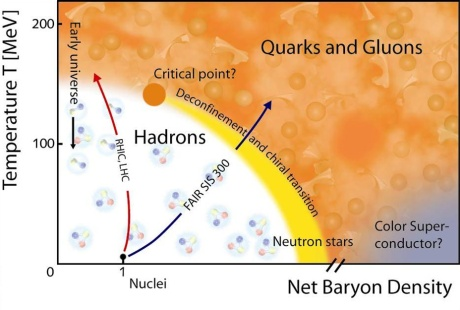
\includegraphics[width=.6\textwidth]{figures/qcd-phase-diagram.png}
  \caption[QCD phase diagram.]{QCD phase diagram. From \cite{Scherer2004}.}
  \label{fig:qcd-phase-diagram}
\end{figure}

Naturally, if one were to study the properties of a substance like e.g.\ H$_2$O one would investigate its phases. The same reasoning applies to the \gls{qgp}: Mapping out the phase diagram will allow us to study quarks and gluons directly as they are described by \gls{qcd}.


\subsection{Nuclear Modification Factor $R_{AA}$}
\label{sec:nuc_mod_factor}

It is very common in heavy ion studies to compare an observable $\Psi_{pp}$ measured in  \gls{pp} collisions to the same quantity measured in \gls{pA} or \gls{AA} collisions with respect to the centrality described by the impact parameter $b$, pseudo rapidity $\eta$\footnote{Pseudo rapidity is defined as $\eta = -\ln\left[\tan\left(\frac{\theta}{2}\right)\right]$ where $\theta$ describes rotations around an axis perpendicular to the beam axis.}, center-of-mass energy $\sqrt{s}$, momentum transverse to the beam axis \pt, and particle type (by mass $m$). If this comparison is carried out by taking the ratio
\begin{equation}
  \label{eq:nuc_mod_factor}
  R_{AA} =
  \frac{\Psi_{AA}(b, \eta, \sqrt{s}, \pt, m)}
  {\left< N_{bin} \right>\Psi_{pp}(b, \eta, \sqrt{s}, \pt, m)}
\end{equation}
$R_{AA}$ (or $R_{pA}$, which is inferred in the following for the sake of brevity) is referred to as \emph{Nuclear modification factor}. If no collective effects were present in \gls{AA} collisions one could regard every such collision as a superposition of pp collisions (\emph{binary scaling}). Therefore, $R_{AA}$ would also depend on the size of the nucleus - an undesirable effect hindering comparisons. To overcome this, $R_{AA}$ is normalized to the mean number of binary collisions between nuclei $\left< N_{bin} \right>$. While $\left< N_{bin} \right>$ is clearly $1$ in case of pp collision it is not a trivial task to determine it for \gls{AA} or \gls{pA} collisions. Commonly, these values are determined by the Glauber-model. With the normalization in place, $R_{AA}$ can either indicate a suppression ($R_{AA} < 1$) or an enhancement ($R_{AA}> 1$) of the respective observable. 

The binary scaling is, however, only applicable if no collective effects are present and hence breaks down for soft parton interactions. The significance of the $R_{AA}$ is thus limited to hard interactions above $\sim \SI{5}{GeV/c}$.

\subsection{ Jet Quenching}
\label{sec:jet-quenching}

One of the most important results in heavy ion physics is the nuclear modification factor of the charged particle density per \pt bin ($\frac{dN_{ch}}{d\pt}$). Current results for \gls{pPb} and \gls{PbPb} collisions are presented in \cite{Abelev2013} and depicted in fig. \ref{fig:RAA}. The \gls{pPb} results are consistent with unity (binary scaling to \gls{pp}) which indicates the absence of a strongly interacting medium in this collision system. The \gls{PbPb} data is presented for central\footnote{While this parameter is naturally available in simulations it has to be inferred from the collision's multiplicity in experimental data. See sec. \ref{sec:mult_classes}} and peripheral collisions revealing a dependence on this impact parameter while both spectra are suppressed over the entire \pt range. The rich structure of the \gls{PbPb} spectrum indicates the presence of the \gls{qgp} which is believed to cause an effect called \emph{jet quenching}: A colored particle of high \pt created within the \gls{qgp} will have to traverse the strongly interacting medium surrounding it. Thereby it loses energy by interacting with the colored medium and will eventually produce a less energetic jet (with smaller multiplicity) than it would have without a medium. The centrality dependence reflects that this effect depends on the size of the medium traversed: Peripheral collisions create a smaller overlap region and thus a smaller \gls{qgp} (if any) compared to central collisions.

\begin{figure}
  \centering
  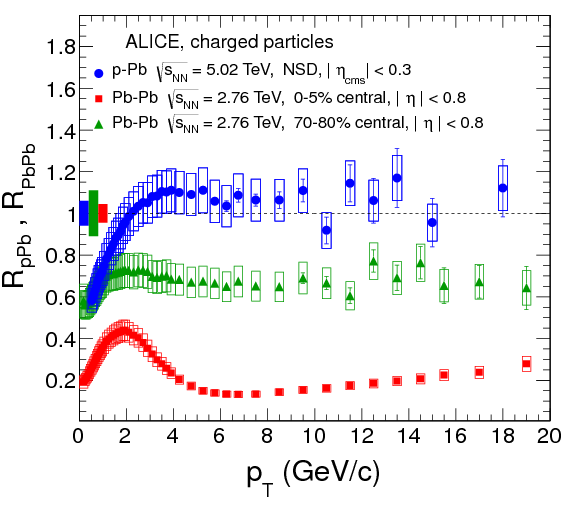
\includegraphics[width=.6\textwidth]{figures/RAA_pPb_PbPb_Alice.png}
  \caption[Nuclear modification factor of charged particle densities for p-Pb, central Pb-Pb and peripheral Pb-Pb collisions.]{Nuclear modification factor of charged particle densities for p-Pb, central Pb-Pb and peripheral Pb-Pb collisions. p-Pb exhibits a suppression for soft events and a binary scaling for $\pt > \SI{2}{GeV/c}$. The Pb-Pb results display a clear centrality dependence. From \cite{Abelev2013}.}
  \label{fig:RAA}
\end{figure}

\subsection{Quarkonium disassociation}
\label{sec:quarkonium}

Another fascinating effect of the \gls{qgp} is the so called ``melting'' of exited states of quarkonium (heavy quark-antiquark pairs). Each excited state exhibits a specific binding energy and is thus expected to break at a unique temperature. Therefore, studying the suppression of these states in heavy ion collisions yields an excellent tool for probing the properties of the created matter. Such studies were carried out for the exited states of $\Upsilon$ ($b\bar{b}$-meson) in \cite{Chatrchyan2011} and confirmed the expectations (cf. fig. \ref{fig:upsilon_suppression}): the exited states $\Upsilon(2S)$ and $\Upsilon(3S)$ were found to be suppressed in \gls{PbPb} collision in comparison to \gls{pp} collisions, again indicating the presence of a strongly interacting medium in \gls{PbPb} collisions.

\begin{figure}
  \centering
  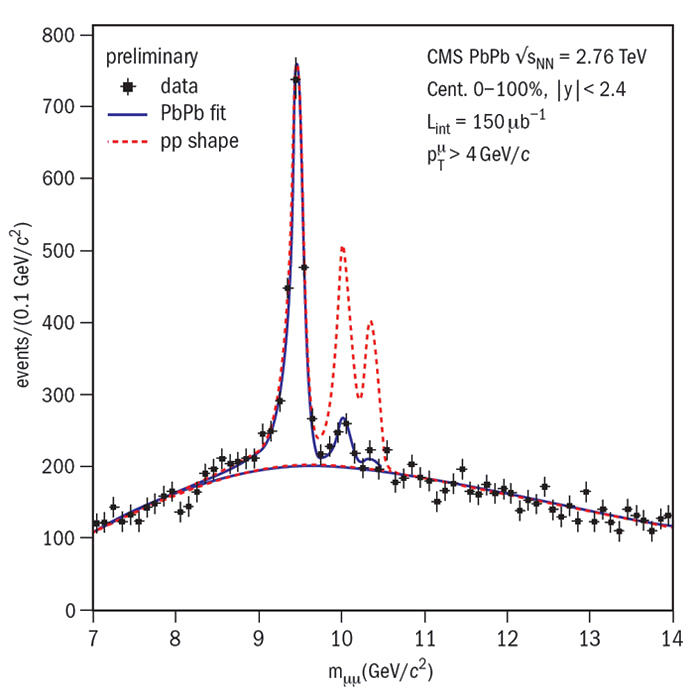
\includegraphics[width=.6\textwidth]{figures/upsilon.jpg}
  \caption[Di-muon invariant mass spectrum from Pb-Pb collisions revealing the suppression of the exited states $\Upsilon(2S)$ and $\Upsilon(2S)$.]{Di-muon invariant mass spectrum from Pb-Pb collisions revealing the suppression of the exited states $\Upsilon(2S)$ and $\Upsilon(2S)$ in comparison to the pp collisions. From \cite{Velkovska2012}.}
  \label{fig:upsilon_suppression}
\end{figure}

\subsection{Hydrodynamic Flow}
\label{sec:flow}

The phenomena of greatest interest for the remainder of this thesis is, however, an anisotropy in the detected particle distribution commonly referred to as \emph{flow}. The effect is observed in the angular correlations\footnote{See sec. \ref{sec:correlation_function} for details on how to obtain these correlations} between a set of two particles which is depicted in fig. \ref{fig:PbPb_2d_flow} (left). Two ridge like structures are visible,  which are elongated over the entire \deta region and are thus called \emph{long-range} correlation. They indicate that the particle production in \gls{PbPb} collisions is enhanced within a plane parallel to the beam axis. The orientation of this plane is different for each event, i.e.\ tilted by an angle $\varphi$ parallel to the beam axis.

\begin{figure}
  \centering
  \begin{subfigure}[m]{0.5\textwidth}
    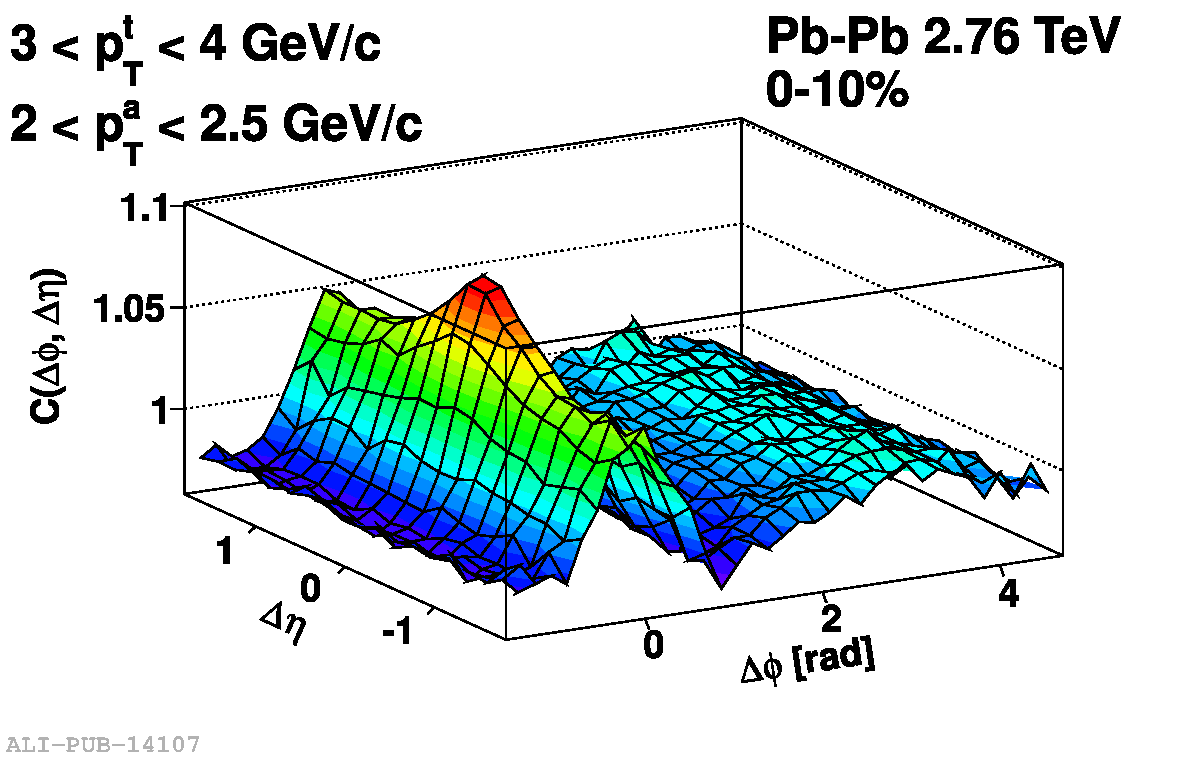
\includegraphics[width=\textwidth]{figures/flow_PbPb_2d.pdf}
  \end{subfigure}%
  \begin{subfigure}[m]{0.5\textwidth}
    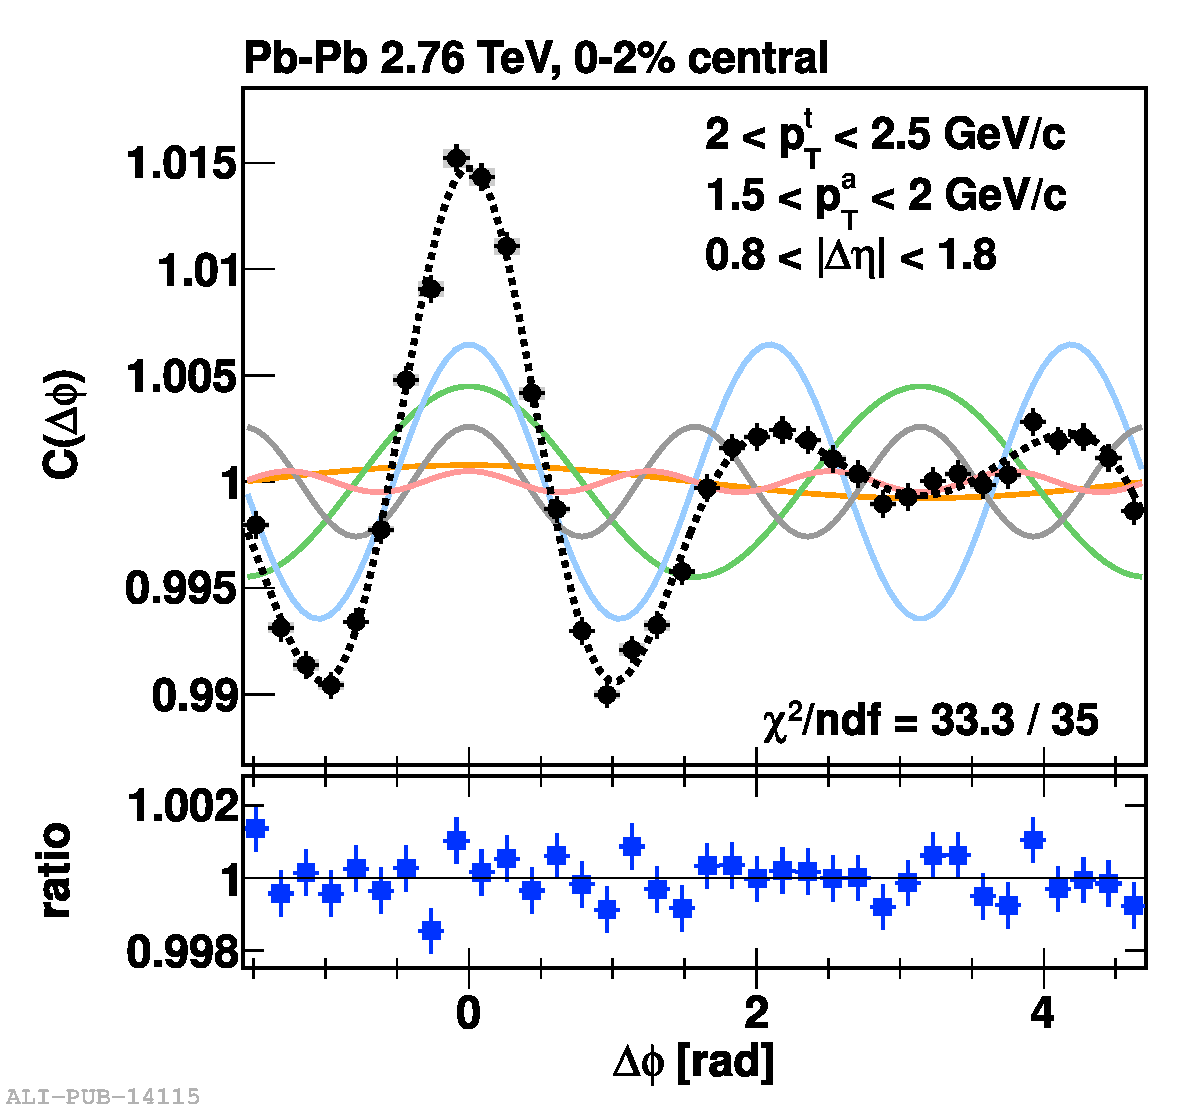
\includegraphics[width=\textwidth]{figures/flow_PbPb_decomp.pdf}
  \end{subfigure}
  \caption[Two-particle correlation functions for Pb-Pb collisions at \SI{2.76}{TeV} at $0-10\%$ centrality and $0-2\%$ centrality.]{Two-particle correlation functions for Pb-Pb collisions at \SI{2.76}{TeV} at $0-10\%$ centrality (left) and $0-2\%$ centrality (right). Left: The Particle production is clearly enhanced along $\dphi = 0$ and $\dphi = \pi$. Right: The two-particle correlation was projected onto \dphi and decomposed into its Fourier components revealing strong contributions of triangular (blue) and elliptic (green) flow. From \cite{Adare2012_2d,Adare2012}.}
  \label{fig:PbPb_2d_flow}
\end{figure}

\begin{figure}
  \centering
  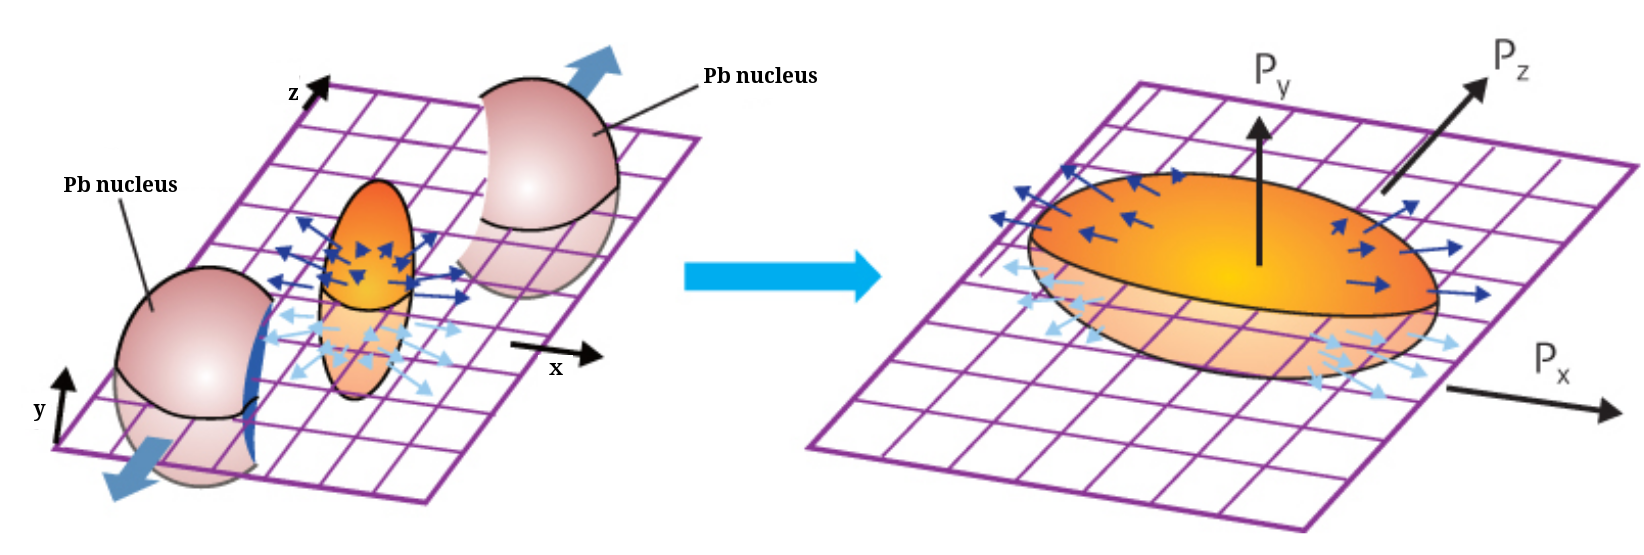
\includegraphics[width=\textwidth]{figures/flow.png}
  \caption[Non central collision result in a ellipsoidal overlap region.]{Non central collision result in a ellipsoidal overlap region. The resulting pressure gradient along the reaction plane leads to an enhancement in hadron production and \pt in-plane compared to out-of-plan.}
  \label{fig:flow_scheme}
\end{figure}


This effect can be very well described by a hydrodynamical expansion of the \gls{qgp}. While the previously described jet-quenching primarily depended on the size of the \gls{qgp}, flow depends on its anisotropic shape. Approximating the two colliding Pb nuclei as spherical objects yields an almond shaped interaction region depending on the impact parameter. Fig. \ref{fig:flow_scheme} (left) depicts such a non-central collision. The hydrodynamical model assumes that the temperature and pressure in the overlap region permit the creation of a \gls{qgp}. The elliptic shape gives then rise to a pressure gradient which will boost particle production and their \pt within the plane depicted as a grid in the figure. This plane is known as the \emph{reaction plane} and is tilted with respect to the laboratory's x-axis by the angle $\Psi^{RP}$.  Assuming a near-ideal Fermi liquid (vanishing viscosity) it is then possible to model the observed azimuthal collective behavior as \cite{Wojciech2010}
\begin{equation}
  \label{eq:flow}
  \frac{dN}{d\eta d^2\pt} = 
  \frac{dN}{2\pi \pt d\pt d\eta} 
  \left[ 1+ \sum_{k=1}^{\infty}2v_k \cos (k(\varphi - \Psi_{k}^{RP})) \right ]
\end{equation}
where $\varphi$ represents the azimuthal angle and $v_k$ is the $k$-th Fourier coefficient depending on $\eta$ and $\pt$. If both nuclei were identical and free of fluctuations, all the odd moments of eq. (\ref{eq:flow}) would vanish \cite{Bozek2010}. Since this is, however, a rather crude approximation, $v_1$ (\emph{direct flow}) and $v_3$ (\emph{triangular flow}) are indeed observed, each in their own reaction plane (angle) $\Psi_k^{RP}$.  However, the \emph{elliptic flow}  $v_2$, which is responsible for the above described boost of particle production within its reaction plane, is the most dominant term in eq. (\ref{eq:flow}) for all but the most central collisions where the almost spherical overlap region favors $v_3$. Fig. \ref{fig:PbPb_2d_flow} (right) displays the Fourier decomposition of such central events. As anticipated, $v_2$ and $v_3$ are the most dominant components.\\

For the case of \gls{PbPb} collisions it was found that the hydrodynamical description of the \gls{qgp} is in excellent agreement to experimental observations for various centralities as well as center-of-mass energies\cite{Manly2006}. Further experimental support for this model is given by the observation of a significant momentum anisotropy for both, light and heavy, hadrons \cite{dEnterria2007}. This suggests a collective behavior of quarks of various flavors prior to hadronization. 

%Collective behavior among the \gls{soft} particles produced in 

%soft QGP, explain with PbPb
%Describe only the phenomenon, no hydro. v2 and v3
%Flow like stuff observed in pPb
%Remainder are possible theoretical models:


\section{Flow like observations in p-Pb collisions}
\label{sec:flow-like-pPb}

It should be emphasized that the hydrodynamic model and the subsequent hadronization is a soft process based on collective behavior of a bulk of strongly interacting particles. It can only be applied if a \gls{qgp}-like medium was formed and if an initial anisotropy is present. While both of these requirements are reasonably likely to be fulfilled in PbPb collisions this cannot be said in the case of \gls{pPb} collisions. Nevertheless, as shown in this thesis as well as in \cite{Abelev2012}, a so-called  \emph{double-ridge} structure can be found in high multiplicity \gls{pPb} collisions. The full procedure for the extraction of this double ridge is exhaustively explained in chapter \ref{chap:methods} but may be summarized (and simplified) as follows: At first, two-particle correlations are calculated for low and high multiplicity events separately (cf. fig. \ref{fig:double_ridge_pPb} top left and bottom left). Both of these correlation functions are dominated by the di-jet component from hard interactions which, it is conjectured, can be removed by subtracting the low multiplicity histogram from the high multiplicity one (fig. \ref{fig:double_ridge_pPb} (right)). This procedure reveals that a flow like double ridge structure is present in high multiplicity events. 

\begin{figure}
  \centering
  \begin{subfigure}[m]{.4\textwidth}
    \begin{subfigure}[b]{\textwidth}
      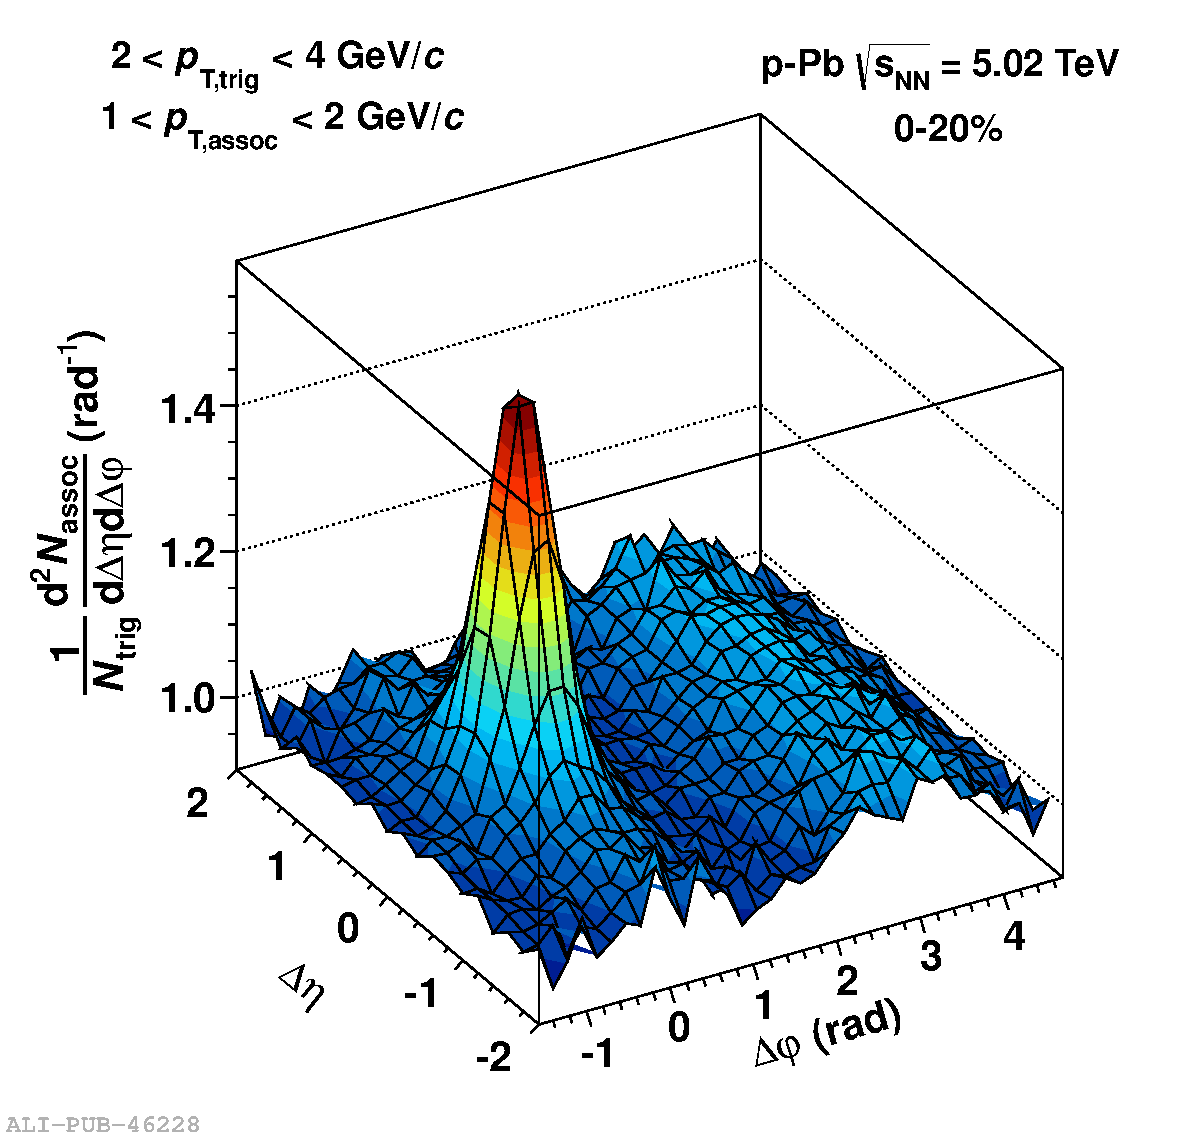
\includegraphics[width=\textwidth]{figures/ty_cent_exampel.pdf}
    \end{subfigure}
    \begin{subfigure}[b]{\textwidth}
      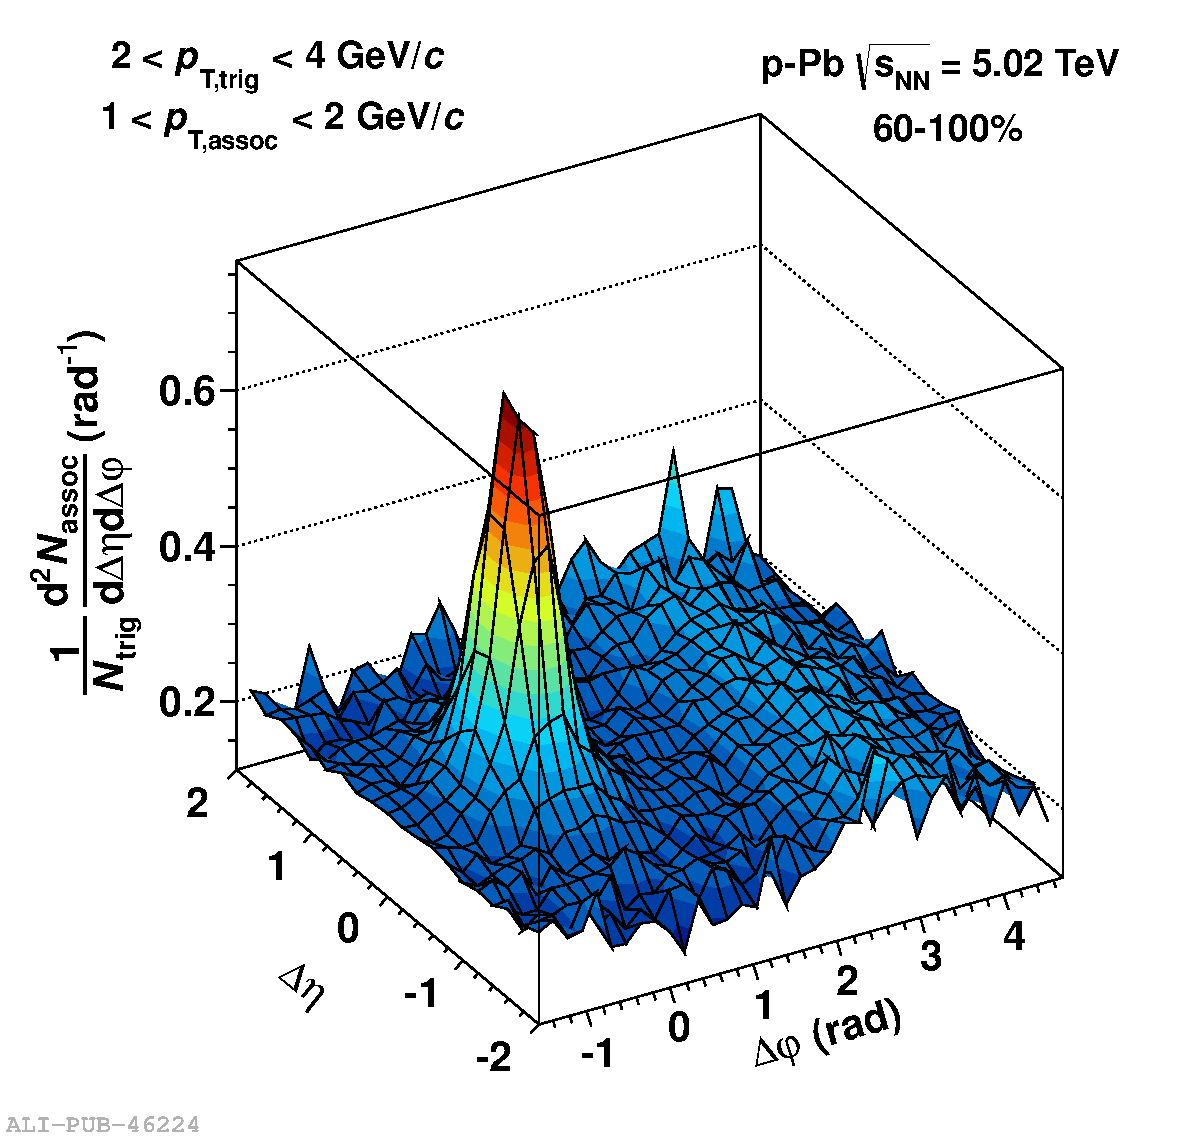
\includegraphics[width=\textwidth]{figures/ty_peri_exampel.pdf}
    \end{subfigure}
  \end{subfigure}%
  \begin{subfigure}[m]{.6\textwidth}
    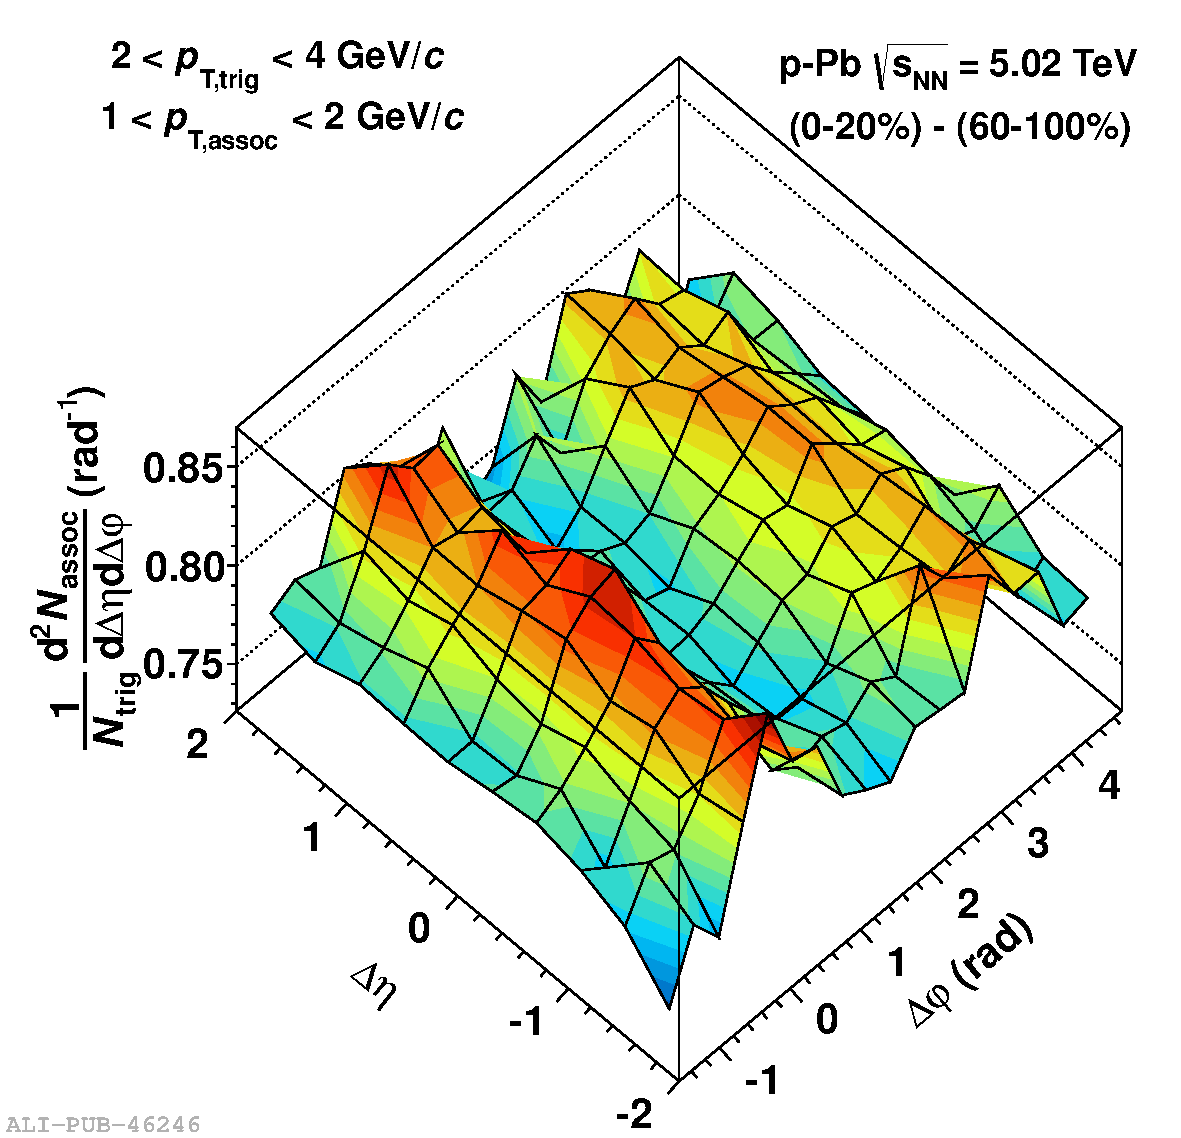
\includegraphics[width=\textwidth]{figures/ty_sub_exampel.pdf}
    %\missingfigure{total yield high multi, total yield low multi and subtraction. Arranged like: http://cms.web.cern.ch/news/unexplained-long-range-correlations-observed-ppb-collisions}
  \end{subfigure}
  \caption[Extraction of the double-ridge structure from pPb measured data at $\sqrt{s}=\SI{5.02}{TeV}$.]{Extraction of the double-ridge structure from pPb measured data at $\sqrt{s}=\SI{5.02}{TeV}$ by calculating the two-particle correlations of high (top left) and low (bottom left) multiplicity events separatly. A subtraction of the two reveals the presence of a flow-like effect in the high multiplicity events. From\cite{Grosse2012_cent,Grosse2012_peri,Grosse2012_sub}.}
  \label{fig:double_ridge_pPb}
\end{figure}

The observation of these long-range \deta correlations was not anticipated but is of great interest and has likely wide ranging consequences for the further understanding of \gls{qcd} effects. Several theoretical explanations have been proposed ranging from final state effects, such as the above described hydrodynamical expansion, to initial state effects modeled by the \gls{cgc} and to hadronization ``cross talk'' between independent partonic collisions described by \emph{Color Reconnection}.

The hydrodynamical model is based on the \gls{qgp} and was described above; the latter two models will be introduced in the following.


\subsection{Color Glass Condensate and Glasma}
\label{sec:CGC}

The \gls{cgc} is a framework for describing the initial states of the colliding hadrons at ultra-relativistic energies. A thorough introduction is presented in \cite{Gelis2013}. Firstly, it takes into account the Lorentz contraction of the nuclei which makes them appear essentially as two dimensional planes in the laboratory frame. Secondly, all the processes which take place within the hadron exhibit a strong time dilation. This makes the partons unlikely to interact with each other during the collision; thus they may be regarded as free. The time dilation does, however, also affects the random fluctuations within the hadron, extending their lifetimes over the duration of the collision. Thus, the gluon density within the nuclei increases with increasing center-of-mass energy. The energies reached by the \gls{lhc} are sufficiently large that the gluons are the main constituents.

Giving this description of the initial states the name of the theory seems aptly: \emph{Color} refers to the color charge of the gluons in the sheets. \emph{Glass} describes the comparably slow time evolution of the constituents and \emph{condensate} refers to the high particle density \cite{Wojciech2010}. This description only applies below a certain momentum scale denoted \emph{saturation momentum} $Q_S$. For momentum transfers much larger than this scale individual gluons can again be resolved.

The collision of two nuclei in this framework is depicted in fig. \ref{fig:cgc_sketch} (left). In the model of \gls{cgc} the two contracted nuclei pass through one another creating a form of matter called \emph{glasma} in between them. If the energy and particle density is large enough, the glasma can produce the \gls{qgp} which may than be subsequently described by the hydrodynamic model.

\begin{figure}
  \centering
  \begin{subfigure}[m]{0.5\textwidth}
    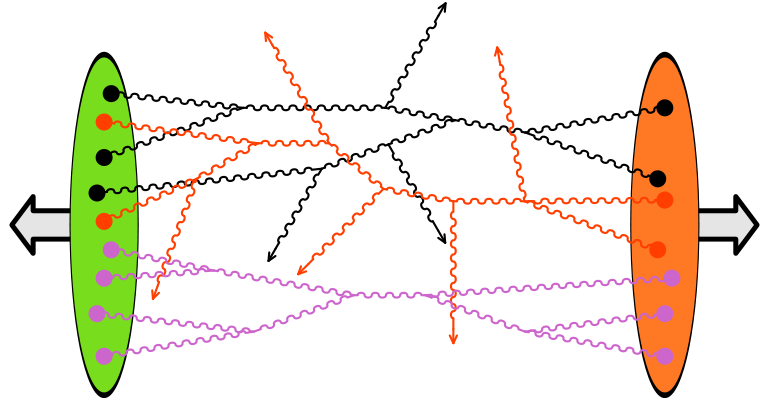
\includegraphics[width=\textwidth]{figures/glasma.png}
  \end{subfigure}%
  \begin{subfigure}[m]{0.5\textwidth}
  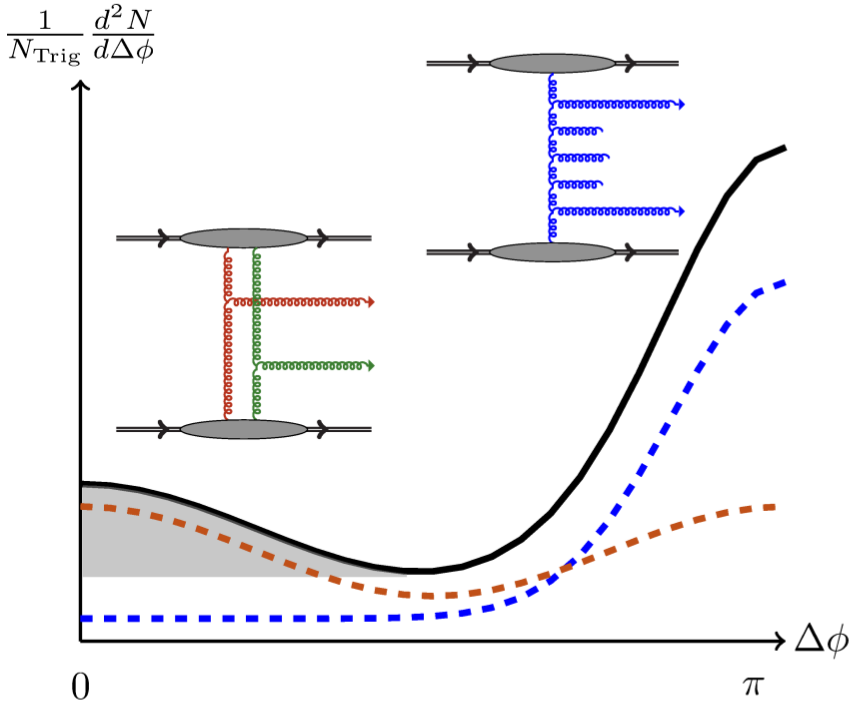
\includegraphics[width=2.95in]{figures/cgc_sketch.png}
  \end{subfigure}
  \caption[Sketch of a di hadron collision in the color glass condensate picture.]{Sketch of a di hadron collision in the color glass condensate picture. Left: Two Lorentz contracted nuclei pass through each other in a collision creating a glasma between each other. Right: The BFKL theory yields a di-ject structure (blue) while the glasma-graph produces a multiplicity dependent double ridge (red). The observed combination of the two processes is shown in black. From \cite{Dusling2012,Gelis2013}.}
  \label{fig:cgc_sketch}
\end{figure}

However, as stated above, it is not at all certain that a \gls{qgp} is created in p-Pb collisions. Thus, an alternative evolution of the glasma yielding a flow-like structure in central collisions is required. In \cite{Dusling2013} the authors claim to have found such a process, or rather the combination of two, recreating the observed p-Pb phenomena. Both processes, sketched in fig. \ref{fig:cgc_sketch} (right), are based on gluon interferences and are referred to as \emph{glasma graphs} and \emph{Balitsky–Fadin–Kuraev–Lipatov (BFKL) dynamics}. The latter describes the di-jet contributions which are only very weakly dependent on the events multiplicity and thus cancel each other when subtracting the two multiplicity classes. The former, on the other hand, yields the elliptic flow like contribution with its symmetry around $\dphi = \pi / 2$ for high multiplicity events.

\subsection{Color reconnection}
\label{sec:CR}
Both the hydrodynamical and the \gls{cgc} model rely on the creation of a medium (either \gls{qgp} or glasma) immediately after the collision which in its own is still disputed. Even if such a creation takes place it arises certain contradictions: eg.\ The interaction of a particle with a medium requires that the mean free path is smaller than the system size. Hence, a model describing collective effects while not relying on a strongly interacting medium is desirable. Such an approach is proposed in \cite{Ortiz2013} based on previous work (see references): Flow like effects in events with multiple hard subcollisions may be produced by minimizing the length of \emph{Lund color strings} by reconnecting final parton from independent hard scatterings. 
\begin{figure}
  \centering
  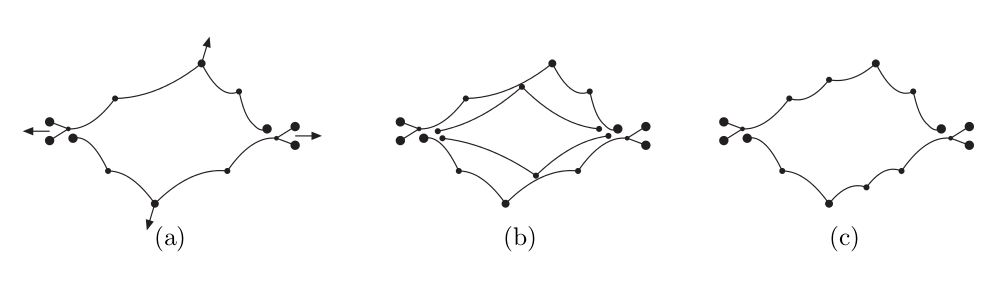
\includegraphics[width=.8\textwidth]{figures/CR.png}
  \caption[Illustration explaining the Color Reconnection taking place for two colliding nuclei.]{Illustration explaining the Color Reconnection taking place for two colliding nuclei. (a) depicts a single hard scattering where the outgoing partons are still color connected to the remnants of the nuclei. Two independent hard scatterings are shown in (b). (c) presents the color reconnected strings. (From \cite{Gustafson2009})}
  \label{fig:cr}
\end{figure}

The effect, labeled as \gls{cr}, is schematically described in fig. \ref{fig:cr}. (a), which depicts a possible string connection for a single hard scattering between two nuclei. The mid-rapidity, back-to-back created partons experience only a small rapidity boost since they are still connected to the remaining nuclei. If, however, multiple hard scatterings were to occur (fig. \ref{fig:cr}b), the strings can  reconnect in a way to minimize the total string length (fig. \ref{fig:cr}c). This reconnection also minimizes the connection to the remaining nuclei and thus increases the mid-rapidity boost of the scattered partons.\\

Fig. \ref{fig:cf_comparison} depicts the dependence of $\left< \pt \right>$ on the charged particle multiplicity $N_{ch}$ for experimental data as well as various event generators for \gls{pp}, \gls{pPb} and \gls{PbPb}. The hydrodynamic based EPOS generator was able to reproduce the \gls{pPb} and \gls{pp} data to a high degree which is surprising since it is based on a hydrodynamic model which should not hold in these systems. Results from the PYTHIA event generator with \gls{cr} are not yet available for \gls{pPb} but this generator was also very successful in describing the \gls{pp} data. However, in contrast to EPOS it did not contradict its underlying model in the process. Of all the listed generators only EPOS and PYTHIA with \gls{cr} yield the potential to reproduce the double ridge in \gls{pPb} data. Hence, this is a strong motivation to further investigate the possibility of applying CR to \gls{pPb} collisions.

\begin{figure}
  \centering
  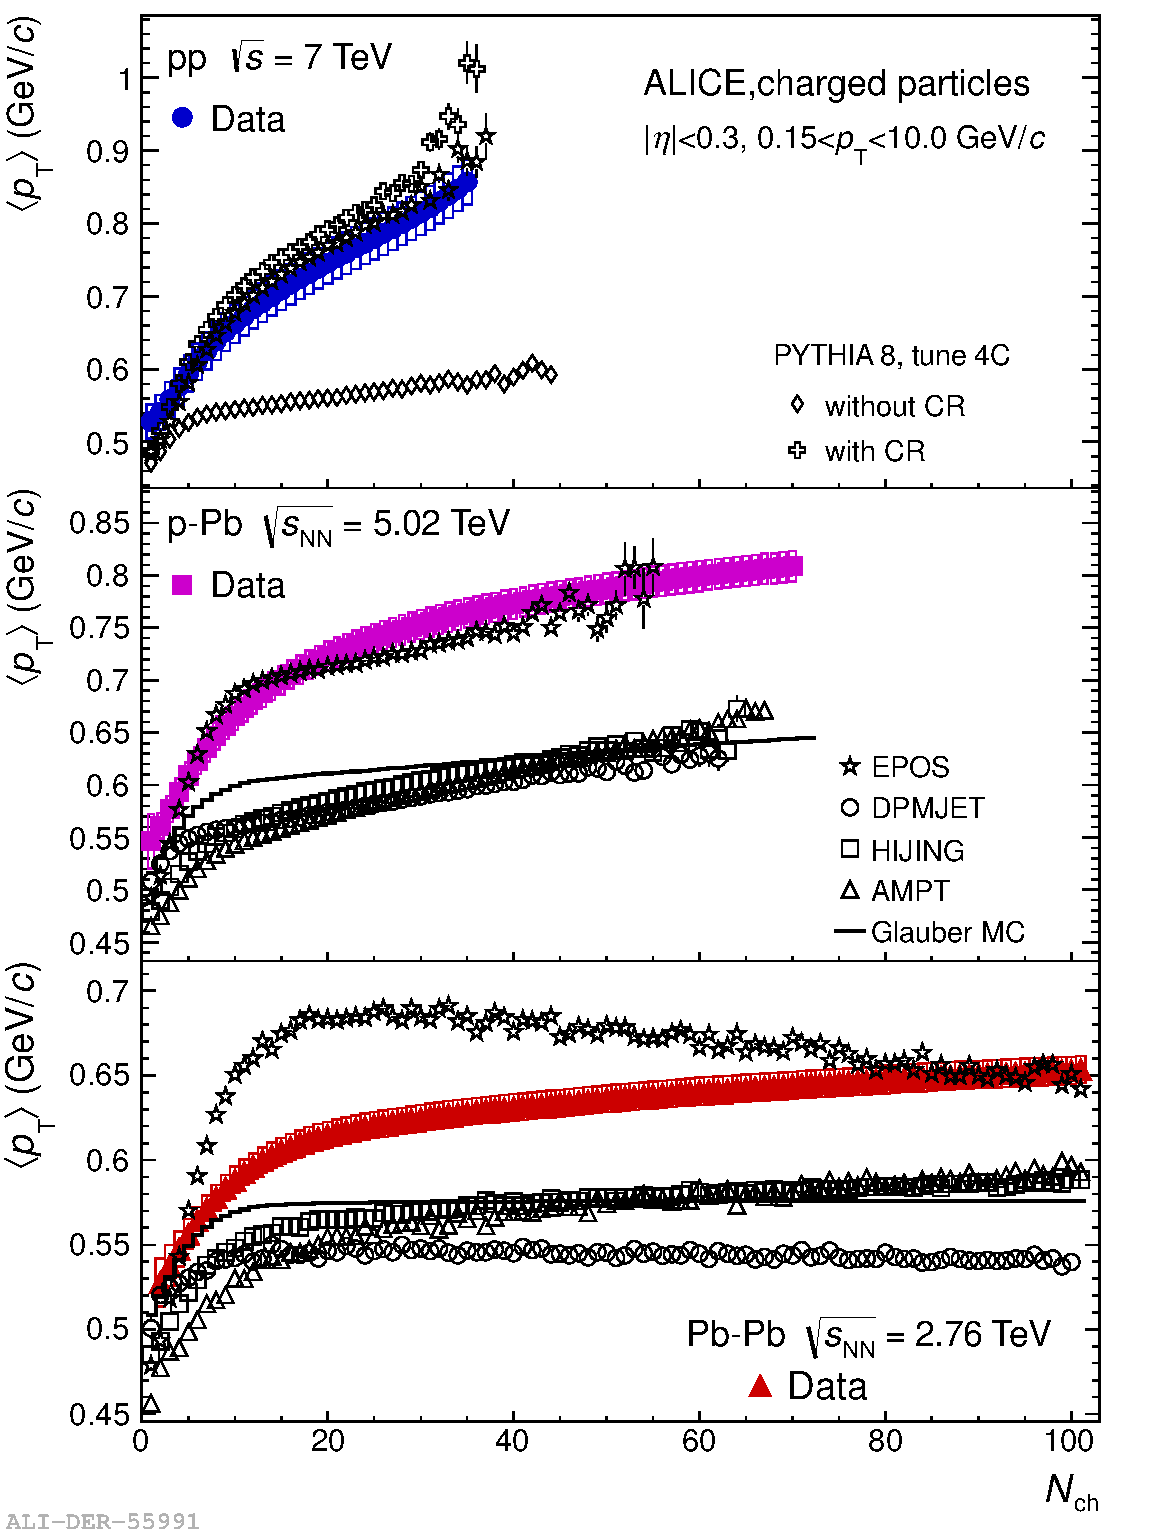
\includegraphics[width=0.6\textwidth]{figures/cr_comparisons.pdf}
  \caption[Mean transverse momentum $\left< \pt \right>$ as a function of charged particle multiplicity $N_{ch}$ for \gls{pp} \gls{pPb} and \gls{PbPb} collisions in comparison to various models.]{Mean transverse momentum $\left< \pt \right>$ as a function of charged particle multiplicity $N_{ch}$ for \gls{pp} \gls{pPb} and \gls{PbPb} collisions in comparison to various models. The Color Reconnection performed competitively to the hydrodynamics based EPOS model. From \cite{cr_epos}.}
  \label{fig:cf_comparison}
\end{figure}


\subsection{Investigating the Double Ridge in Soft and Hard Events}
\label{sec:hard-soft}

It is important to note that all of the above proposed explanations have fundamentally different concepts if and what medium is created in the collisions. The hydrodynamical model depends on the presents of the \gls{qgp}, the \gls{cgc} of its glasma and the \gls{cr} expects no medium at all. Thus, these theories are in principle mutually exclusive and it is of great importance to falsify or confirm any of these models. 

As discussed in sec. \ref{sec:prob-sm}, it is common to refer to individual subcollisions or particle tracks as \emph{hard} and \emph{soft} but this classification may also be applied to entire events. \cite{Acosta2002} studied antiproton-proton ($\bar{\text{p}}\text{p}$) collisions while applying such an event discrimination. An event was classified as hard if a single calorimeter cluster was above $\SI{1}{GeV}$ transverse energy ($E_{\text{T}}$) and soft otherwise. The analysis revealed large differences between the two samples. Fig. \ref{fig:soft_hard_example} displays the $\left< \pt \right>$ as a function of charged particle multiplicity for different center-of-mass energies $\sqrt{s}$. The shape of the distributions as well as the scaling with $\sqrt{s}$ are evidently dependent on the soft and hard event classification.
\begin{figure}
  \centering
  \begin{subfigure}[b]{0.45\textwidth}
    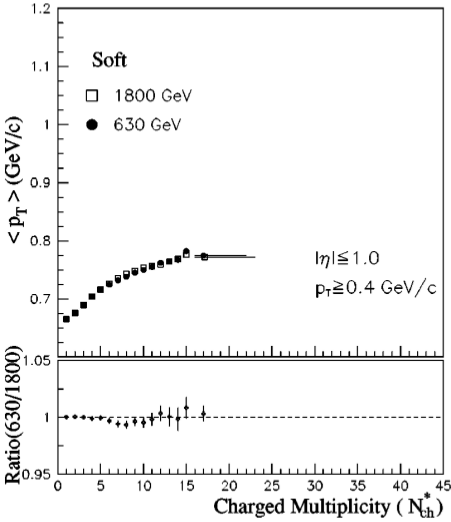
\includegraphics[width=\textwidth]{figures/soft_mult_pt.png}
  \end{subfigure}
  \begin{subfigure}[b]{0.45\textwidth}
  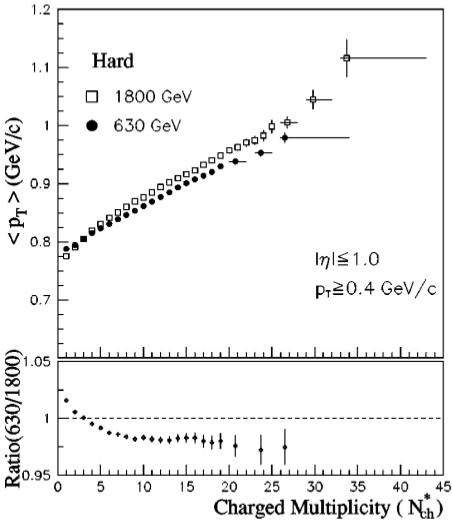
\includegraphics[width=\textwidth]{figures/hard_mult_pt.png}
  \end{subfigure}
  \caption[Mean transverse momentum $\left< \pt \right>$ vs. charged particle multiplicity $N_{ch}$ at center-of-mass energies $\sqrt{s}$ of $\SI{630}{GeV}$ and $\SI{1800}{GeV}$.]{Mean transverse momentum $\left< \pt \right>$ vs. charged particle multiplicity $N_{ch}$ at center-of-mass energies $\sqrt{s}$ of $\SI{630}{GeV}$ and $\SI{1800}{GeV}$. The event sample was divided into soft (left) and hard (right) events each exhibiting distinct results. From \cite{Acosta2002}.}
    \label{fig:soft_hard_example}
\end{figure}

A similar disjunction of the event sample was carried out in this analysis probing the dependence of the double ridge structure on the hardness of the underlying events. The three discussed models are expected to behave as follows under the introduction of a bias towards harder events:
\begin{description}
\item [Hydrodynamical expansion] is expected to show no dependence on the hardness of an event since the underlying \gls{qgp} is a soft effect and will not interact with hard high \pt particles.
\item [Glasma] is only descriptive of interaction with momentum transfer below the saturation value $Q_S$ which lies in the range of $1.6$ to $\SI{1.9}{GeV/c}$. Thus, the glasma should not show a dependence on the hardening of the event sample either.
\item [Color Reconnection] on the other hand, is a process build around the interplay of hard interactions. Thus, if \gls{cr} is responsible for the observed double ridge in \gls{pPb} data, one can expect modifications of it by biasing the event sample to harder events.
\end{description}

%%% Local Variables: 
%%% mode: latex
%%% TeX-master: "main"
%%% End: 
